\documentclass[xcolor=pdftex,dvipsnames,table,mathserif]{beamer}
%\usepackage{subfigure}
\usepackage{amsbsy}
\usepackage{tikz}
\usetikzlibrary{arrows}
\usepackage{amsmath,graphicx,dsfont,color}
\usepackage{amsfonts}
\usepackage{amssymb}
\usepackage{array}

\usepackage{subfig}

% makes the subfig package work
\makeatletter
\let\@@magyar@captionfix\relax
\makeatother

% subfigure counter resets every frame
\makeatletter
\@addtoreset{subfigure}{framenumber}
\makeatother

% First author and year
\bibliographystyle{apalike}

% This sets the list items of the bibliography to the same symbol used for citation.
\setbeamertemplate{bibliography item}{\insertbiblabel}

% This avoids extralines for different entries
\setbeamertemplate{bibliography entry title}{}
\setbeamertemplate{bibliography entry location}{}
\setbeamertemplate{bibliography entry note}{}

\DeclareMathOperator*{\argmin}{arg\,min}
\DeclareMathOperator*{\argmax}{arg\,max}
%Definitiona

\newcommand{\x}{\mathbf{x}}
\newcommand{\X}{\mathbf{X}}
\newcommand{\W}{\mathbf{W}} %Weight
\newcommand{\bais}{\mathbf{b}}%Bais
\newcommand{\act}{\texttt{g}}%Activation
\newcommand{\loss}{L}
\newcommand{\pdata}{\hat{p}_{\texttt{data}}}
\newcommand{\nsize}{N}
\newcommand{\nfeatures}{P}
\newcommand{\param}{\boldsymbol{\theta}}
\newcommand{\featmap}{\boldsymbol{\phi}}
\newcommand{\EV}{\mathbb{E}}







\usepackage{physics}

\graphicspath{{../graphics/}}

\AtBeginSection[]{
  \begin{frame}{Contents}
  \tableofcontents[currentsection, hideothersubsections]
  \end{frame}
}

\AtBeginSubsection[]{
  \begin{frame}{Contents}
  \tableofcontents[currentsection, subsectionstyle=show/shaded/hide]
  \end{frame}
}

\setbeamertemplate{footline}[frame number]{}
\setbeamertemplate{navigation symbols}{}
\setbeamertemplate{section in toc}[square]
\setbeamertemplate{items}[square]

\title{Practical recommendations}
\author{E. Decencière}
\date{MINES ParisTech\\
  PSL Research University\\
  Center for Mathematical Morphology
}
\titlegraphic{
\includegraphics[height=1.7cm]{../graphics/logoemp}}

\useinnertheme{rounded}
\usecolortheme{rose}

%%%%%%%%%%%%%%%%%%%%%%%%%%%%%%%%%%%%%%%%%%%%%%%%%%%%%%%
%%%%%%%%%%%%%%%%%%%%%%%%%%%%%%%%%%%%%%%%%%%%%%%%%%%%%%%

\begin{document}

\frame{\titlepage}

\frame{
\frametitle{Contents}
\tableofcontents[hidesubsections]
}

%%%%%%%%%%%%%%%%%%%%%%%%%%%%%%%%%%%%%%%%%%%%%%%%%%
%%%%%%%%%%%%%%%%%%%%%%%%%%%%%%%%%%%%%%%%%%%%%%%%%%
\section{Introduction}


%%%%%%%%%%%%%%%%%%%%%%%%%%%%%%%%%%%%
\begin{frame}{Recall from previous days}

\end{frame}



%%%%%%%%%%%%%%%%%%%%%%%%%%%%%%%%%%%%%%%%%%%%%%%%%%
\section{Problem representation}

%%%%%%%%%%%%%%%%%%%%%%%%%%%%%%%%%%%%%%%%%%%%%%%%%%%%%
\frame{
  \frametitle{Modeling your problem}

  \begin{block}{Casting your problem into the right representation}
    \begin {itemize}
    \item Familiarize yourself with the training data (input and output images)
    \item Choose the right representation for your images
    \item Choose an architecture and train it
    \item Analyze the results on the validation data (\alert{look} at the images!)
    \item Do you need preprocessing? Data augmentation? Post-processing?
    \item Iterate ...
    \item Only at the end: test!
    \end{itemize}

  \end{block}

}


%%%%%%%%%%%%%%%%%%%%%%%%%%%%%%%%%%%%%%%%%%%%%%%%%%%%%
\section{Data preparation}


%%%%%%%%%%%%%%%%%%%%%%%%%%%%%%%%%%%%
\begin{frame}{Building the datasets}
  \begin{itemize}
  \item Gather your images in order to build a dataset that conveniently represents your problem
  \item How many images do you need?
  \item Build a proper ground-truth
  \end{itemize}

  \begin{alertblock}{Is database constitution de main step?}
    \begin{itemize}
    \item In practical, real-world applications, this is becoming to most time-consuming step
    \item If the dataset does not conveniently represent your problem you will run into difficulties
    \end{itemize}

\end{alertblock}

\end{frame}

%%%%%%%%%%%%%%%%%%%%%%%%%%%%%%%%%%%%
\begin{frame}{Anecdote: tank detection}

  In the first years of artificial neural networks, a perceptron was trained to detect images containing tanks. Its results were quite good...

  \pause

  ... but in fact images containing tanks were acquired during sunny days, while images without tanks were shot with overcast weather. The network was simply detecting lighter images!

  \pause

  (This anecdote might be a urgan legent, but nevertheless is a good illustration of the problems one might run into during database preparation)
\end{frame}

%%%%%%%%%%%%%%%%%%%%%%%%%%%%%%%%%%%%%%%%%%%%%%%%%%%%%
\frame{
  \frametitle{What quality is needed for the ground-truth?}

  \begin{itemize}
  \item Deep learning models tend to be robust with respect to ground-truth errors
  \item In the case of segmentation, you do not need a pixel-precision high quality segmentation
  \end{itemize}

}

%%%%%%%%%%%%%%%%%%%%%%%%%%%%%%%%%%%%%%%%%%%%%%%%%%%%%
\frame{
  \frametitle{Preprocessing}

  \begin {itemize}
  \item Standard statistical preprocessing: not always useful, and sometimes problematic, when applied to images
    \item Morphological operators
  \end{itemize}

}


%%%%%%%%%%%%%%%%%%%%%%%%%%%%%%%%%%%%%%%%%%%%%%%%%%%%%
\frame{
  \frametitle{Data augmentation}

  \begin {itemize}
\item Geometrical transformations: similarities
\item Elastic transformations
\item Specific methods: articulated objects, \ldots
\item Simulated data
  \end{itemize}

}



%%%%%%%%%%%%%%%%%%%%%%%%%%%%%%%%%%%%%%%%%%%%%%%%%%%%%
\section{Examples}

%%%%%%%%%%%%%%%%%%%%%%%%%%%%%%%%%%%%%%%%%%%%%%%%%%%%%
\begin{frame}{Astronomy}
    \begin{columns}[c]
    \column{.5\textwidth}
        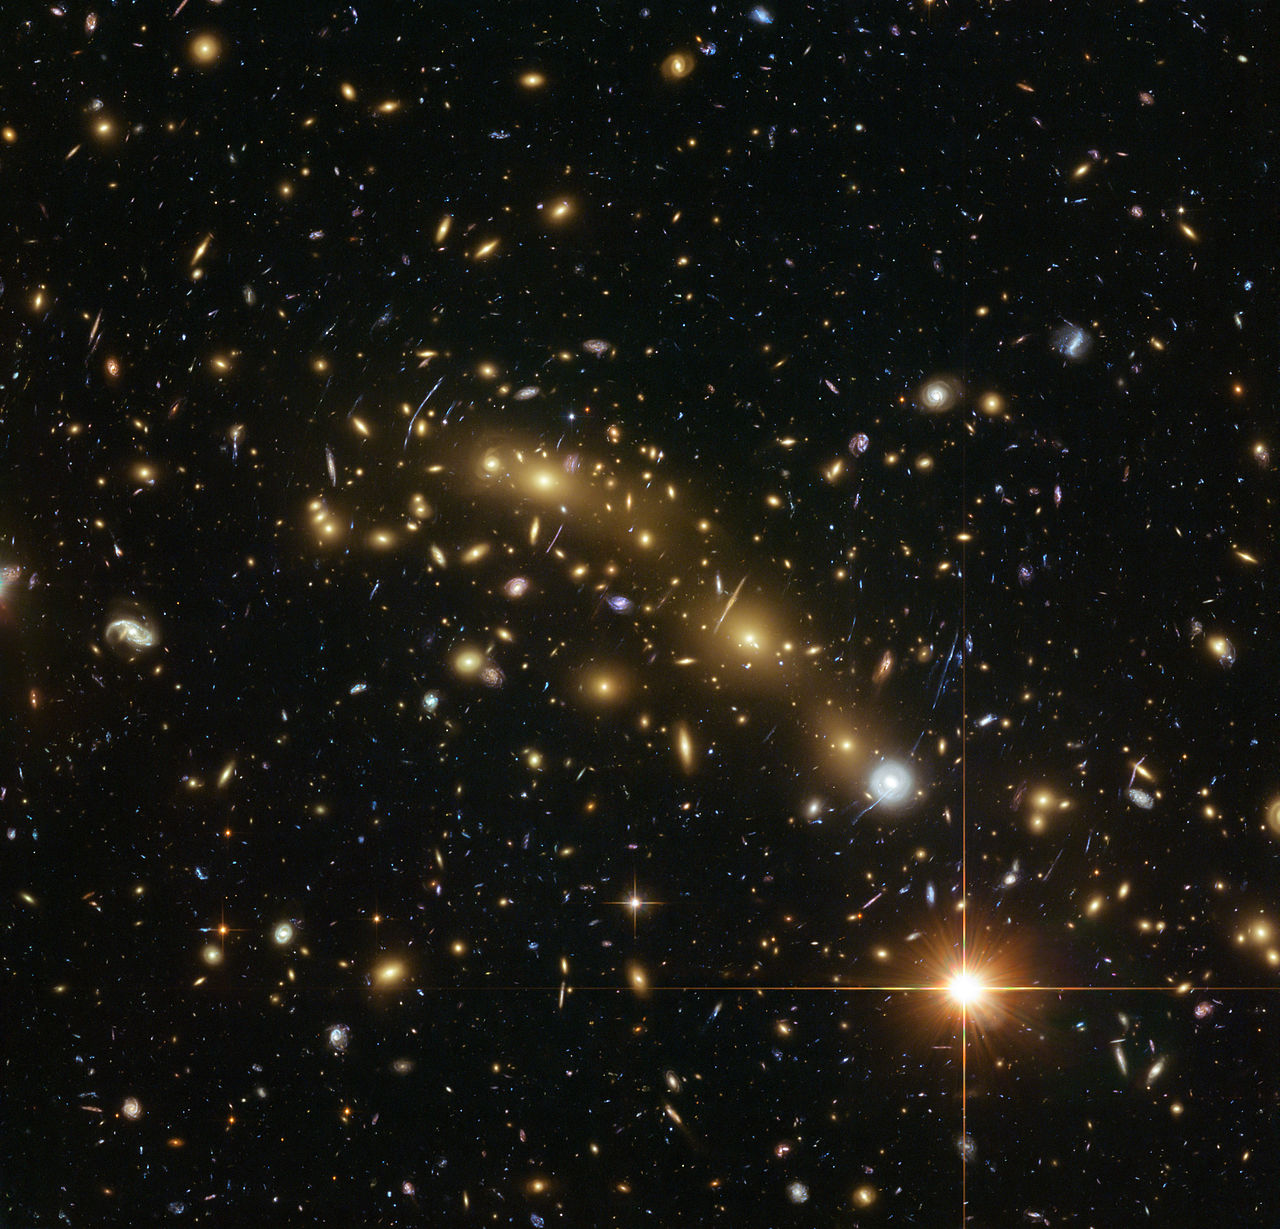
\includegraphics[width=0.9\textwidth]{hst.jpg}\\
        {\tiny (Credits: ESA/Hubble, CC BY 4.0, https://commons.wikimedia.org/w/index.php?curid=34205833)}
    \column{.5\textwidth}
      How would you:
      \begin{itemize}
      \item segment the background?
      \item segment the sources?
      \item separate the sources?
      \end{itemize}

    \end{columns}
\end{frame}



%%%%%%%%%%%%%%%%%%%%%%%%%%%%%%%%%%%%%%%%%%%%%%%%%%

%%%%%%%%%%%%%%%%%%%%%%%%%%%%%%%%%%%%%%%%%%%%%%%%%%
\section*{References}

%%%%%%%%%%%%%%%%%%%%%%%%%%%%%%%%%%%%%%%%%%%%%%%%%%

\frame[allowframebreaks]{

\scriptsize

\frametitle{References}

%\bibliographystyle{amsalpha}
%\bibliographystyle{apalike}

\bibliography{edf.bib}

\normalsize

}




\end{document}
